\documentclass[xetex,mathserif,serif]{beamer}
\usepackage{polyglossia}
\setdefaultlanguage[babelshorthands=true]{russian}
\usepackage{tabu}
\usepackage{pgfplots}
\usepackage{textpos}

\useoutertheme{infolines}

\usepackage{fontspec}
\setmainfont{FreeSans}
\newfontfamily{\russianfonttt}{FreeSans}

\usepackage{forest}
\usetikzlibrary{arrows}

\newcommand{\attribution}[1] {
	\vspace{-5mm}\begin{flushright}\begin{scriptsize}\textcolor{gray}{\textcopyright\, #1}\end{scriptsize}\end{flushright}
}

\tabulinesep=0.7mm

\title{О разработке программных продуктов}
\author[Юрий Литвинов]{Юрий Литвинов \newline \textcolor{gray}{\small\texttt{yurii.litvinov@gmail.com}}}

\date{08.10.2019}

\begin{document}
	
	\frame{\titlepage}
	
	\begin{frame}
		\frametitle{Программа и программный продукт}
		\begin{center}
			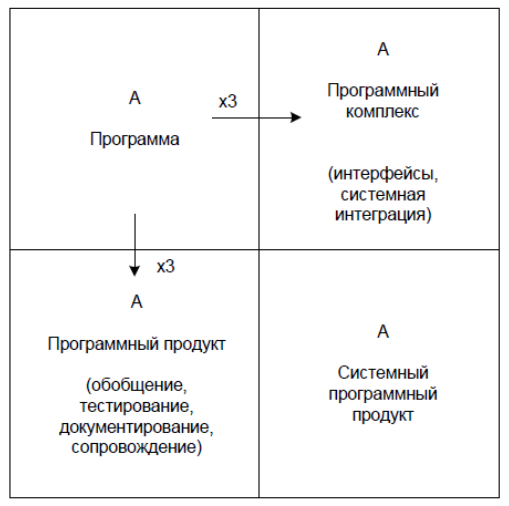
\includegraphics[width=0.5\textwidth]{mythical-man-month.png}
		\end{center}
		\begin{center}
			Ф. Брукс, ``Мифический человеко-месяц''
		\end{center}
	\end{frame}

	\begin{frame}
		\frametitle{Жизненный цикл ПО}
		\begin{itemize}
			\item Последовательность стадий
			\begin{itemize}
				\item Состав и последовательность работ
				\item Получаемые результаты
				\item Методы и средства
				\item Роли и ответственности
				\item ...
			\end{itemize}
		\end{itemize}
	\end{frame}

	\begin{frame}
		\frametitle{Фазы жизненного цикла ПО}
		\begin{itemize}
			\item возникновение и исследование идеи
			\item анализ и сбор требований
			\begin{itemize}
				\item пилотный проект
			\end{itemize}
			\item планирование и проектирование
			\item разработка
			\item отладка и тестирование
			\item сдача
			\item сопровождение
			\item вывод из эксплуатации
		\end{itemize}
	\end{frame}

	\begin{frame}
		\frametitle{Водопадная модель}
		\begin{center}
			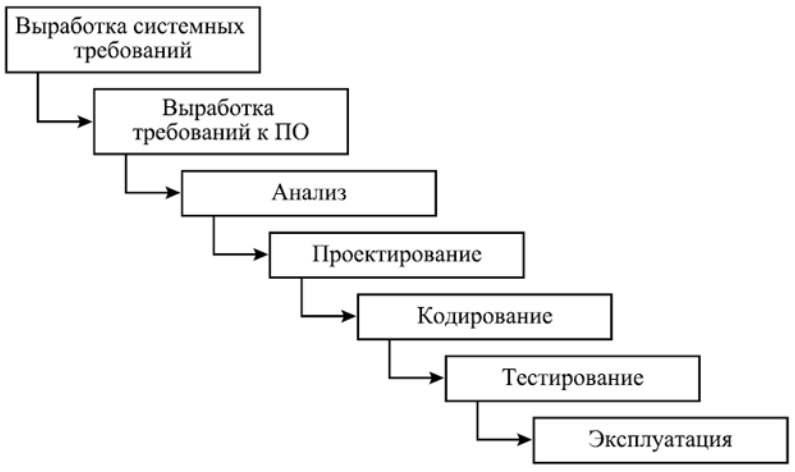
\includegraphics[width=0.7\textwidth]{waterfall-model.png}
		\end{center}
	\end{frame}

	\begin{frame}
		\frametitle{Спиральная модель}
		\begin{center}
			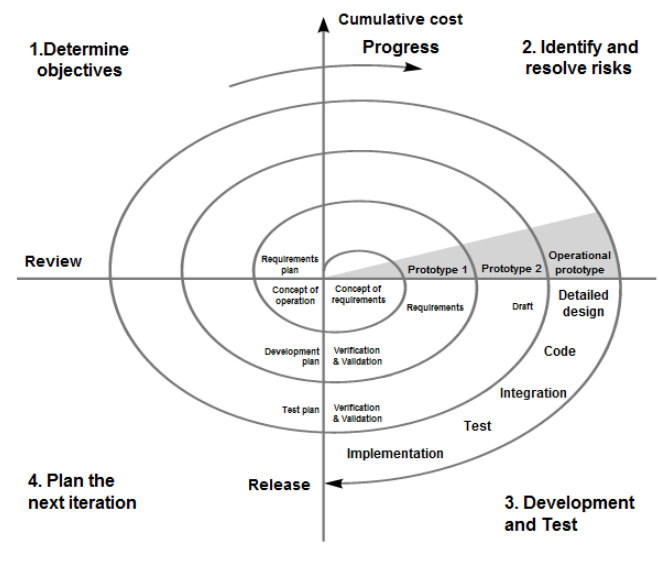
\includegraphics[width=0.7\textwidth]{spiral-model.png}
		\end{center}
	\end{frame}

	\begin{frame}
		\frametitle{Методологии разработки}
		\begin{itemize}
			\item Модели описывают последовательность фаз и что надо делать на этих фазах, методологии --- как делать
			\item Гибкие методологии
			\begin{itemize}
				\item Agile Manifesto
				\begin{itemize}
					\item Люди и взаимодействие важнее процессов и инструментов
					\item Работающий продукт важнее исчерпывающей документации
					\item Сотрудничество с заказчиком важнее согласования условий контракта
					\item Готовность к изменениям важнее следования первоначальному плану
				\end{itemize}
				\item SCRUM
				\item XP
			\end{itemize}
		\end{itemize}
	\end{frame}

	\begin{frame}
		\frametitle{Парадигмы программирования}
		\begin{itemize}
			\item Методологии говорят, как делать, но до уровня ``а сейчас писать код'', стиль написания кода --- выбранная парадигма
			\item Структурное программирование
			\item Объектно-ориентированное программирование
			\item Функциональное программирование
			\item Много других
		\end{itemize}
	\end{frame}

	\begin{frame}
		\frametitle{Структурное программирование}
		\begin{itemize}
			\item Дейкстра, 70-е годы XX века
			\item Базовые конструкции
			\begin{itemize}
				\item Последовательное исполнение
				\item Ветвление
				\item Цикл
			\end{itemize}
			\item Произвольная вложенность
			\item Никаких других средств управления последовательностью выполнения
			\item Выделение подпрограмм
			\item Нисходящее проектирование
		\end{itemize}
	\end{frame}

	\begin{frame}
		\frametitle{Нисходящее проектирование}
		\begin{itemize}
			\item Декомпозиция задачи
			\begin{itemize}
				\item Подпрограммы
				\item Модули
			\end{itemize}
			\item Высокоуровневая реализация с помощью ``заглушек''
			\item Постепенная реализация модулей и подпрограмм
			\item Строгое задание входов и выходов
		\end{itemize}
	\end{frame}

	\begin{frame}
		\frametitle{Модули}
		\begin{itemize}
			\item Логически обособленный кусок функциональности
			\begin{itemize}
				\item Интерфейс
				\item Реализация
			\end{itemize}
			\item Особенности
			\begin{itemize}
				\item Четкая декомпозиция
				\item Минимизация
				\item Один модуль --- одна функциональность
				\item Отсутствие побочных эффектов
				\item Независимость от реализации других модулей
				\item Принцип сокрытия данных
			\end{itemize}
		\end{itemize}
	\end{frame}

	\begin{frame}
		\frametitle{Практики}
		\begin{itemize}
			\item Документирование
			\item Моделирование
			\item Тестирование (модульное и регрессионное)
			\item Версионный контроль
			\item Непрерывная интеграция
			\item Code review
		\end{itemize}
	\end{frame}

	\begin{frame}
		\frametitle{Версионный контроль}
		\begin{center}
			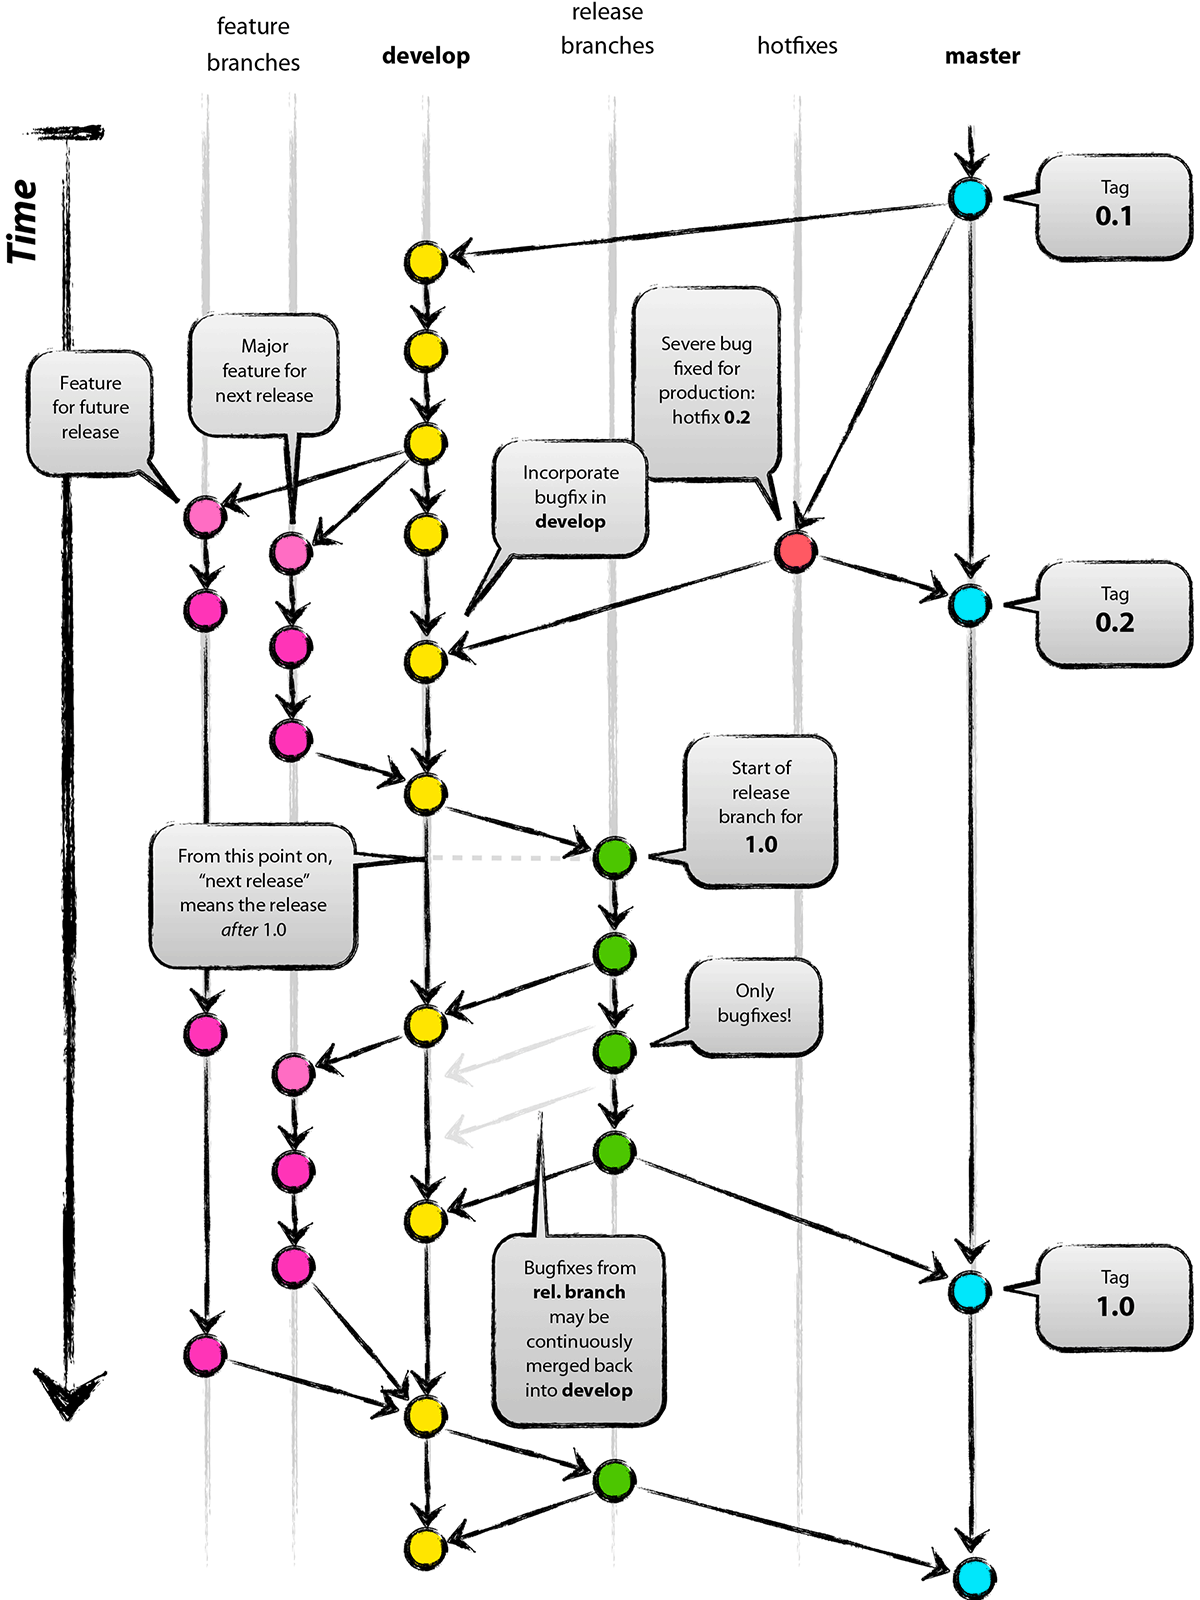
\includegraphics[width=0.42\textwidth]{git-flow.png}
			\attribution{https://nvie.com/posts/a-successful-git-branching-model/}
		\end{center}
	\end{frame}

\end{document}